\chapter{Конструкторский раздел}
В этом разделе приводится подробное описание разрабатываемого метода, выделяются основные его компоненты, описываются метрики, оценивающие метод. В выводах аналитической части предлагается разработать новый метод распределения оперативной памяти приложений. Новый метод будет включать в себя выделение памяти запрашиваемого размера и ее освобождение.

\section{Структура программного комплекса}
\begin{figure}[!h]
	\begin{center}
		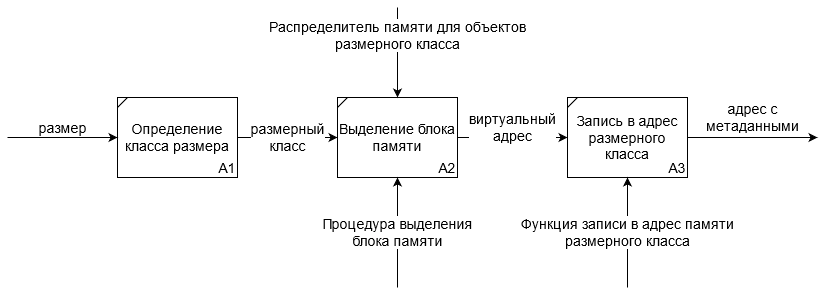
\includegraphics[scale=0.5]{images/block-allocation.png}
		\caption{Выделение блока памяти.}
		\label{block-allocation}
	\end{center}
\end{figure}

\begin{figure}[!h]
	\begin{center}
		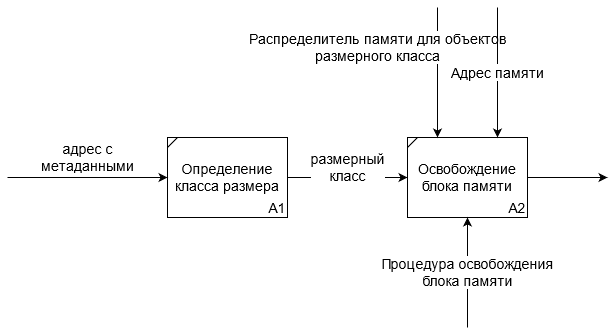
\includegraphics[scale=0.5]{images/block-free.png}
		\caption{Освобождение блока памяти.}
		\label{block-free}
	\end{center}
\end{figure}

Аллокатору передается размер памяти, которую необходимо выделить, в байтах. Далее, в зависимости от того, к какому классу относится размер, есть три варианта выделения памяти:
\begin{itemize}
	\item малые объекты, это объекты размер кототрых менее либо равен 2048-и байтам, они выделяются через специализированный аллокатор для малых объектов;
	\item большие объекты, это объекты размер которых менее либо равен 1МБ по умолчанию, (ограничение может быть изменено, но не должно превышать 268431360 байт) они выделяются через аллокатор для больших объектов;
	\item огромные объекты, класс объектов, размер которых более чем ограничение для больших объектов, такие объекты выделяются сразу через систменый вызов \textbf{mmap}.
\end{itemize}

Результатом запроса в распределитеть памяти является адрес, выровненный по размеру страницы и содержащий в себе всю необходимую информацию для освобождения объекта. После освобождения, память кэшируется в случае для малых и больших запросов. Память под огромные объекты, при освобождениии, сразу возвращается ОС.

Для работы с возвращаемым адресом необходимо использовать функцию \textit{getWorkingAddress}, которая приводит старшие 16 бит к необходимому виду, чтобы не происходил доступ к закрытым адресам.

\begin{lstlisting}
template<typename T>
T *getWorkingAddress(T *value)
{
	static constexpr uint64_t workingAddressMask = (static_cast<uint64_t>(1) << highestVirtualSpaceBit) - 1;
	uint64_t address = reinterpret_cast<uint64_t>(value) & workingAddressMask;
		
	if ((reinterpret_cast<uint64_t>(value) & (static_cast<uint64_t>(1) << (highestVirtualSpaceBit - 1))) != 0)
	{
		static constexpr uint64_t highHalf = static_cast<uint64_t>(0x1ffff) << (highestVirtualSpaceBit - 1);
		address |= highHalf;
	}

	return reinterpret_cast<T *>(address);
}
\end{lstlisting}

\subsection{Основная идея}
Метод основан на использовании старших бит виртуального адреса. На рисунке \ref{64bit-memory-addressing} показана диаграмма перевода виртульного адреса в физический в 64-х битной системе.

\begin{figure}[!h]
	\begin{center}
		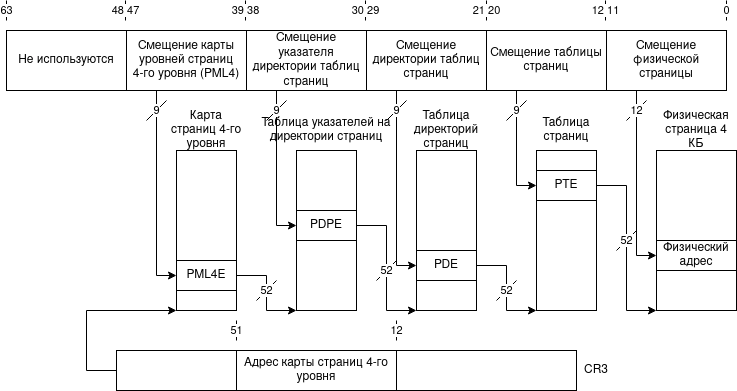
\includegraphics[scale=0.6]{images/64bit-memory-addressing.png}
		\caption{Адресация памяти в 64-х битном режиме.}
		\label{64bit-memory-addressing}
	\end{center}
\end{figure}

Как видно из рисунка \ref{64bit-memory-addressing}, для адресации используются только первые 48 бит из 64-х, остальные 16 бит разграничивают виртуального адресное пространство на зоны нижних и верхних адресов. Биты 63-48 разграничивают знак, если 47-й выставлен в 0, то все верхние 16 тоже выставлены в 0 и такие адреса относятся к нижней половине, если 47-й бит выставлен в 1, то биты 63-48 тоже равны 1 и такие адреса относятся к верхней половине виртульных адресов.\cite{paging}

\begin{figure}[!h]
	\begin{center}
		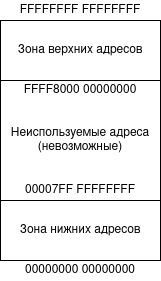
\includegraphics[scale=0.6]{images/48bit-half-spaces.png}
		\caption{48-и битная адресация.}
		\label{48bit-half-spaces}
	\end{center}
\end{figure}

Данная реализация распределителся памяти использует верхние 16 бит виртуального 64-х битного адреса для хранения информации о типе (большой/малый) и размерном классе объекта. При запросе на выделение памяти, в вернувшийся адрес записывается информация о классе объекта, за это отвечают биты 62-48. В самый старший бит записывается тип объекта малый/большой.\cite{page-tables}

\subsection{Аллокатор для малых объектов}
Все запросы на выделение памяти размером менее или равным 2048 байт обслуживаются аллокатором для малых объектов. Для каждого потока создается свой такой аллокатор, при завершении работы потока вся память высвобождается ОС. Объекты должны иметь размер кратный степени 2-и начиная с размера в 8 байт и заканчивая размером 2048 байт. Если на вход приходит размер, который не кратен степени 2-ки, то он приводится к ближаешему больгему размеру кратному степени 2-и. Благодаря такой логике, можно найти подходящий аллокатор для данного размерного класса.

В случае малых объектов, возвращаемому адресу может быть выставлен только один из 15-и старших бит, чтобы можно было точно определить размер объекта при освобождении памяти. Самый старший бит выставляется в 1, чтобы можно было точно определить тип объекта.

\begin{figure}[!h]
	\begin{center}
		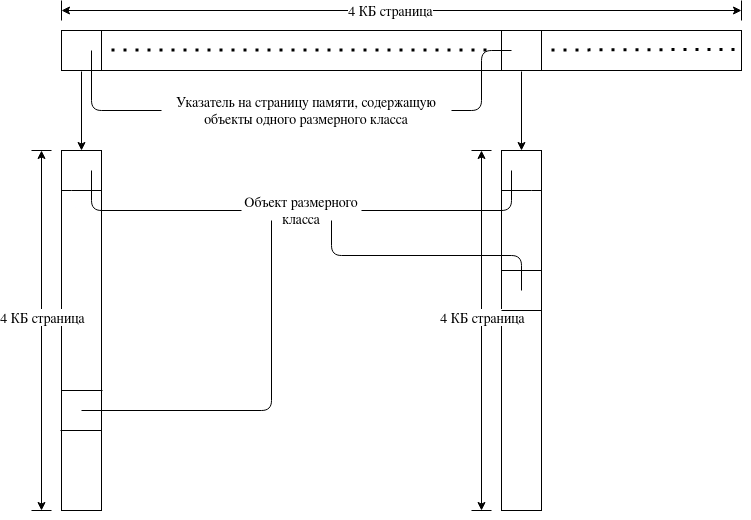
\includegraphics[scale=0.6]{images/small-allocator-design.png}
		\caption{Общий вид аллокатора для малых объектов.}
		\label{small-allocator-design}
	\end{center}
\end{figure}

Реализация аллокатора включает в себя метаданные и указатели на выделенные страницы памяти, где и находятся все объекты. При запросе на выделение, алокатор инициализирует метаданные, размер метаданных в байтах равен одной странице и память выделяется через \textbf{mmap}. Так как в 64-й системе размер указателя равен 8-и байтам, то метаданные могут содержать 512 указателей на страницы с объектами (размер каждой страницы равен 4 КБ, тоесть системному размеру страницы). Когда пользователь запрашивает память, то есть несколько вариантов исполнения запроса:
\begin{itemize}
	\item аллокатор пустой или не был инициализирован, в таком случае будет выделена отдельная страница под класс объектов и польщователю вернется указатель на эту страницу, в метаданные запишется адрес страницы и указатель на свободный элемент сместится на адрес страницы + размерный класс объекта;
	\item аллокатор уже имеет выделенные страницы памяти, в таком случае он попытается выделить память под текузему указателю на свободную память, если тот выходит за пределы доступной памяти, то происходит поиск свободного элемента в той же странице памяти, (это необходимо для того, чтобы не подгружать новые страницы памяти, потому что физический адрес уже был получен и закэширован в буффере ассоциативной трансляции) если же в странице нет свободной памяти, то будет проихведен поиск по всем страницам и будет возвращена первая найденая область памяти и указатель на свободную память выставлен в адрес текущей старницы + размер объекта, но если свободных объектов не оказалось и есть место в метаданных для выделения новой страницы, то выделяется новая страница и возвращается ее адрес, иначе, аллокатор не сможет удовлетворить запрос;
	\item аллокатор переполнен, это означает что используется память под все 512 страниц и все объекты заняты, большей памятью аллокатор управлять не может и программа завершится.
\end{itemize}

Когда пользователь делает запрос на освобождение памяти, то память, которую он передал в аллокатор, заполняется нулями и помечается как свободная. При освобождении, из адреса выделяется тип объекта и его размер, по ним далее идет поиск нужного аллокатора для размерного класса.

\subsection{Аллокатор для больших объектов}
Если размер объекта более чем 2048 байт и менее чем заданное ограничениеили равно ему (по умолчанию 1МБ), то память под объекта выделяется через аллокатор для больших объектов. В данном случае возвращаемому адресу выставляется 63-й бит в 0, что отвечает за большой тип объекта, а в биты 48-62 записывается размерный класс объекта разделенный на размер страницы. Поэтому аллокатор умеет выделять память под объекты, размер которых не может превышать 268431360 байт и каждый такой объект обязан быть кратным размеру страницы.

\begin{figure}[!h]
	\begin{center}
		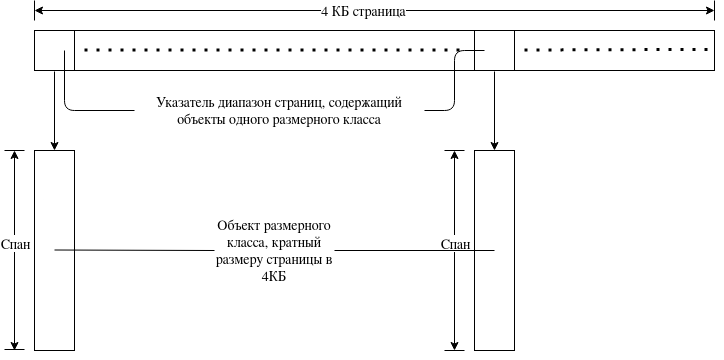
\includegraphics[scale=0.6]{images/large-allocator-design.png}
		\caption{Общий вид аллокатора для больших объектов.}
		\label{large-allocator-design}
	\end{center}
\end{figure}

Разграничение доступа к аллокатору из нескольких потоков осуществляется через спин лок\cite{spinlock}, реализованный через атомарные примитивы, для каждого размерного класса есть свой спин лок.

\begin{lstlisting}
class SpinLock
{
	public:
	SpinLock() noexcept = default;
	SpinLock(const SpinLock &other) : lock_(other.lock_.load()) {}
	SpinLock &operator=(const SpinLock &other)
	{
		lock_.store(other.lock_.load());
		return *this;
	}
	
	void lock() noexcept
	{
		for (;;)
		{
			if (!lock_.exchange(true, std::memory_order_acquire))
			{
				return;
			}
			while (lock_.load(std::memory_order_relaxed))
			{
				__builtin_ia32_pause();
			}
		}
	}
	
	bool tryLock() noexcept
	{
		return !lock_.load(std::memory_order_relaxed) &&
		!lock_.exchange(true, std::memory_order_acquire);
	}
	
	void unlock() noexcept
	{
		lock_.store(false, std::memory_order_release);
	}
	
	private:
	std::atomic<bool> lock_{false};
};
\end{lstlisting}

Реализация аллокатора похожа на реализацию аллокатора для малых объектов, за исключением того, что вместо малых объектов на страницу, в метаданных содержатся указатели на спаны, размер спана равен следующему значению кратному размеру страницы относительно запрашиваемого размера на выделение (только если тот уже не был кратен размеру страницы). В метаданных также могут одновременно находится указатели на 512 объектов определенного размерного класса, но каждый указатель теперь указывает на один объект, а не совокупность, поэтому реализация проще. Когда пользователь делает запрос на выделение памяти, он удовлетворяется по исходя из следующих шагов:
\begin{itemize}
	\item если аллокатор пустой, то выделятся одна страница памяти под метаданные и польщователю отдается указатель на адрес выделенный через вызов \textbf{mmap};
	\item если в аллокаторе уже есть объекты данного размерного класса, то пользователю вернется указатель на последний объект в метаданных, который после удаляется из метаданных.
\end{itemize}

При освобождении памяти работает следующая логика:
\begin{itemize}
	\item если в метаданных не заполнены все элементы, то указатель помещается в конец метаданных;
	\item если аллокатор заполнен (в метаданных уже содержатся 512 элементов), то память возвращается ОС через вызов \textbf{munmap}.
\end{itemize}

\subsection{Аллокатор для огромных объектов}
Если запрашиваемый размер более чем ограничение для больших объектов, то память выделяется сразу через вызов \textbf{mmap} и освобождается через вызов \textbf{munmap}. Для метаданных выделяется страница, которая расположена перед указателем на память под объект, поэтому память в общем случае выделяется размером 4 КБ + следующий размер кратный размеру странице относительно переданного размера. В метаданных хранится размер объекта, чтобы потом передать его в функцию \textbf{munmap}.

\begin{figure}[!h]
	\begin{center}
		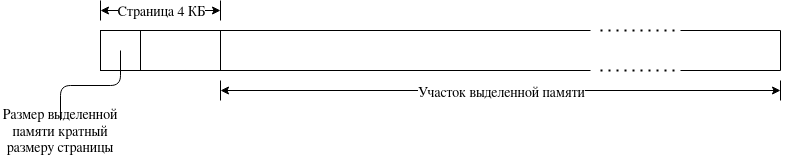
\includegraphics[scale=0.5]{images/huge-allocator-design.png}
		\caption{Общий вид аллокатора для огромных объектов.}
		\label{huge-allocator-design}
	\end{center}
\end{figure}

\pagebreak
\begin{lstlisting}
static auto createSmallObjectsRegistries()
{
	std::array<SmallObjectsRegistry, 9> registries;
	for (uint64_t index{0}, size{smallObjectsSizeStart}; size <= smallObjectsSizeLimit;
	++index, size <<= 1)
	{
		registries[index] = SmallObjectsRegistry{size};
	}
	return registries;
}

static SmallObjectsRegistry &getSmallObjectsRegistry(size_t size)
{
	thread_local auto registries = createSmallObjectsRegistries();
	uint64_t index{0};
	for (; size > smallObjectsSizeStart; size >>= 1, ++index)
	;
	return registries[index];
}

static auto createLargeObjectsRegistries()
{
	static constexpr uint64_t count = largeObjectsSizeLimit / largeObjectsSizeStart;
	std::array<LargeObjectsRegistry, count> registries;
	for (uint64_t index{0}, size{largeObjectsSizeStart}; index < count; ++index, size += pageSiz
	e)
	{
		registries[index] = std::move(LargeObjectsRegistry{size});
	}
	return registries;
}

static LargeObjectsRegistry &getLargeObjectsRegistry(size_t size)
{
	assert(isDivisibleBy<pageSize>(size));
	static auto registries = createLargeObjectsRegistries();
	return registries[size / pageSize - 1];
}

void *malloc(size_t size)
{
	void *ptr{nullptr};
	if (size <= smallObjectsSizeLimit)
	{
		size = roundUpToNextPowerOf2(size);
		auto &registry = getSmallObjectsRegistry(size);
		assert(registry.pop(ptr));
		
		uint64_t controlBits = (size << highestVirtualSpaceBit) | smallObjectMask;
		ptr = reinterpret_cast<void *>(reinterpret_cast<uint64_t>(ptr) | controlBits);
	}
	else
	{
		size = getNextNearestDivisibleByPageSize(size);
		
		if (size <= largeObjectsSizeLimit)
		{
			auto &registry = getLargeObjectsRegistry(size);
			registry.pop(ptr);
			
			uint64_t controlBits = (size / pageSize) << highestVirtualSpaceBit;
			ptr = reinterpret_cast<void *>(reinterpret_cast<uint64_t>(ptr) | controlBits);
		}
		else
		{
			ptr = mmapImpl(pageSize + size);
			*static_cast<uint64_t *>(ptr) = size;
			ptr = static_cast<std::byte *>(ptr) + pageSize;
		}
	}
	return ptr;
}

void free(void *ptr)
{
	uint64_t address = reinterpret_cast<uint64_t>(ptr);
	size_t sizeClass = (address >> highestVirtualSpaceBit) & 0x7fff;
	
	ptr = getWorkingAddress(ptr);
	
	if (sizeClass <= smallObjectsSizeLimit)
	{
		auto &registry = getSmallObjectsRegistry(sizeClass);
		registry.push(ptr);
	}
	else if (sizeClass != 0)
	{
		auto &registry = getLargeObjectsRegistry(sizeClass * pageSize);
		registry.push(ptr);
	}
	else
	{
		ptr = static_cast<std::byte *>(ptr) - pageSize;
		munmapImpl(ptr, *static_cast<uint64_t *>(ptr));
	}
}
\end{lstlisting}